\documentclass[12pt]{article}

% Packages for styling and layout
\usepackage[table,xcdraw]{xcolor}
\usepackage{tikz}
\usepackage{geometry}
\usepackage{graphicx} % Added for image support
\geometry{margin=1in}

% Custom colors for tidal force
\definecolor{darkgrey}{RGB}{64,64,64}
\definecolor{maroon}{RGB}{128,0,0}

% Title styling
\newcommand{\teamtitle}{
    \centering
    \begin{tikzpicture}
        % Header Image
        \node[draw=none, anchor=north west] at (0, 0) {\includegraphics[width=\textwidth]{resources/Header.png}};

        % Year in top right
        \node[draw=none, text=maroon, font=\large\bfseries] at (16, -1.8) {\the\year};
    \end{tikzpicture}
    \vspace{1em}
}

% Bingo grid dimensions
\newcommand{\bingosize}{5} % 5x5 grid

% Bingo cell styling
\newcommand{\bingocell}[1]{
    \node[draw, thick, minimum size=3cm, align=center] {#1};
}

\begin{document}

\teamtitle

\begin{center}
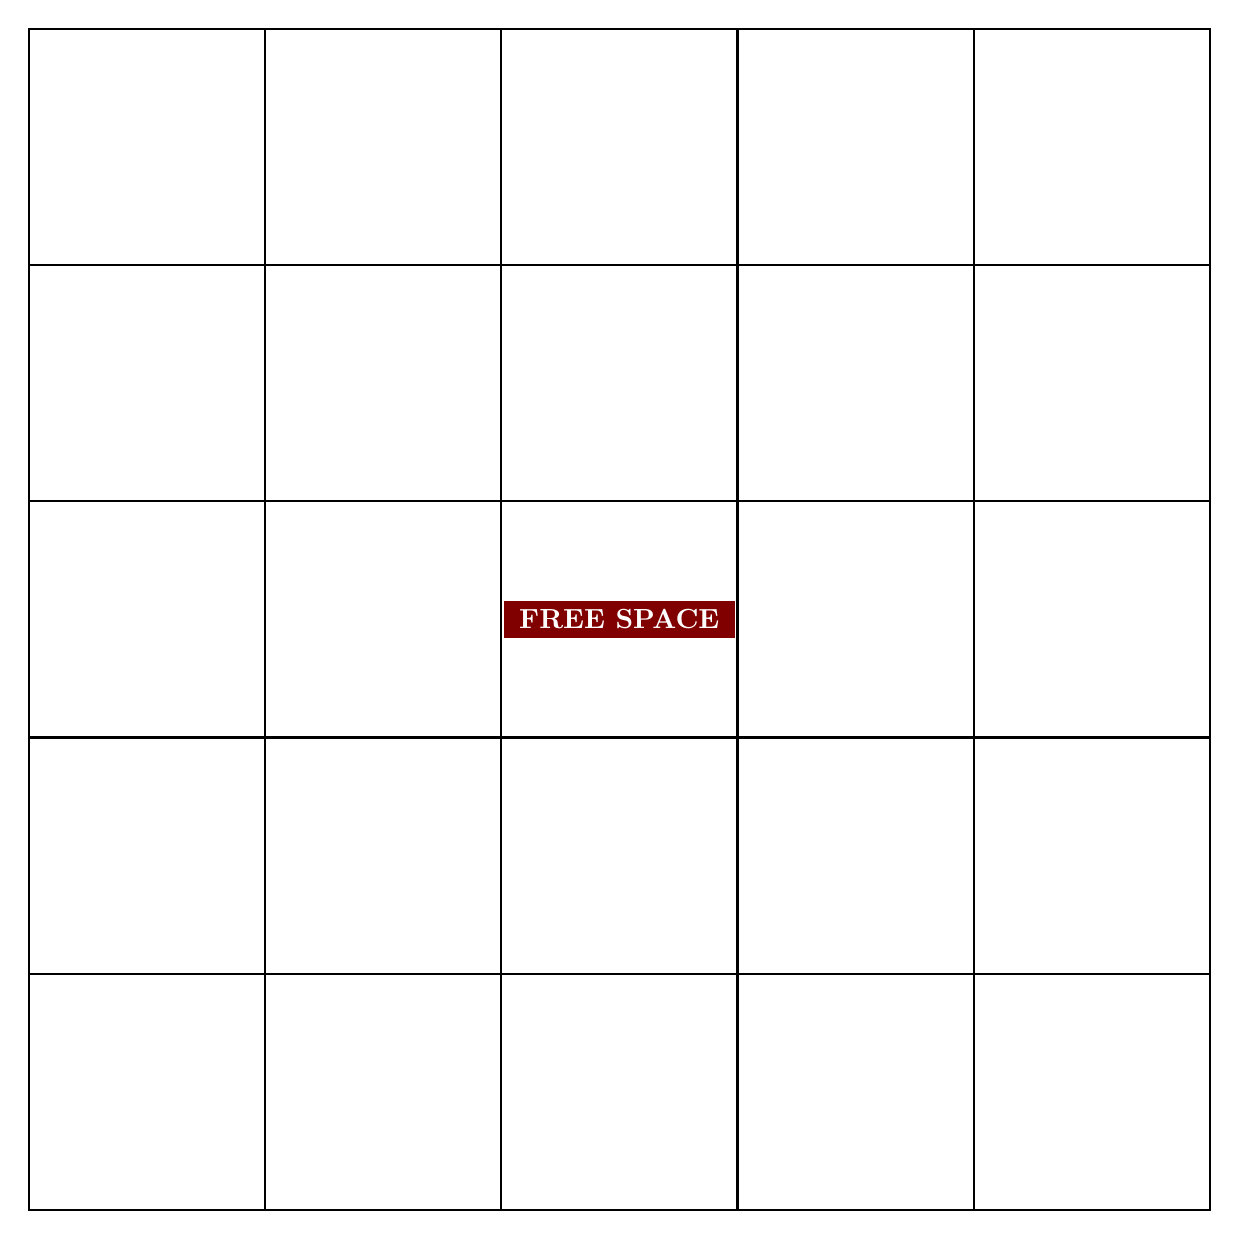
\begin{tikzpicture}[x=3cm, y=3cm]
    % Draw grid
    \foreach \x in {0,...,\numexpr\bingosize-1\relax} {
        \foreach \y in {0,...,\numexpr\bingosize-1\relax} {
            \node[draw, thick, minimum size=3cm, align=center] at (\x, -\y) {\phantom{X}};
        }
    }

    % Static cells
    % Center free space cell light grey background
    \node[fill=maroon, text=white, text width=2.7cm,font=\bfseries, align=center] at (2, -2) {FREE SPACE};

    % 0,2 cell "mentor space" maroon background
    % 4,2 Alumni space, white background


    % \node[thick, text width=3.5cm, align=center] at (1, -1) {Team Stands Around the Broken Robot};

    % {AUTOPOP ANCHOR}

\end{tikzpicture}

\textbf{Rules:} \\
\begin{enumerate}
 \item You must be present and witness the square you mark!
 \item No purposefully causing a square!
 \item Have fun!
\end{enumerate}

\end{center}

\end{document}
